\begin{adjustwidth*}{}{-2.25in}
\textbf{{\large Exercises}}
\setlength{\columnsep}{25pt}
\begin{multicols*}{2}
\noindent Terms and Concepts \small
\begin{enumerate}[1)]
\item T/F: Simpson's Rule is a method of approximating antiderivatives.
\item What are the two basic situations where approximating the value of a definite integral is necessary?
\item Why are the Left and Right Hand Rules rarely used?
\end{enumerate} 

\noindent {\normalsize Problems} \small

\noindent{\bf In exercises 4--11, a definite integral is given.
\ba
\item Approximate the definite integral with $T_4$.
\item Approximate the definite integral with $S_4$.
\item Compute the exact value of the integral.
\ea}

\begin{enumerate}[1),resume]
\item $\ds \int_{-1}^1 x^2\ dx$
\item $\ds \int_{0}^{10} 5x\ dx$
\item $\ds \int_{0}^{\pi} \sin x\ dx$
\item $\ds \int_{0}^{4} \sqrt x\ dx$
\item $\ds \int_{0}^{3} (x^3+2x^2-5x+7)\ dx$
\item $\ds \int_{0}^{1} x^4\ dx$
\item $\ds \int_{0}^{2\pi} \cos x\ dx$
\item $\ds \int_{-3}^{3} \sqrt{9-x^2} \ dx$
\end{enumerate}

\noindent{\bf In exercises 12--19, approximate the definite integral with $T_6$ and $S_6$.}

\begin{enumerate}[1),resume]
\item $\ds \int_{0}^{1} \cos \big(x^2\big) \ dx$
\item $\ds \int_{-1}^{1} e^{x^2} \ dx$
\item $\ds \int_{0}^{5} \sqrt{x^2+1} \ dx$
\item $\ds \int_{0}^{\pi} x\sin x \ dx$
\item $\ds \int_{0}^{\pi/2} \sqrt{\cos x} \ dx$
\item $\ds \int_{1}^{4} \ln x \ dx$
\item $\ds \int_{-1}^{1} \frac{1}{\sin x+2} \ dx$
\item $\ds \int_{0}^{6} \frac{1}{\sin x+2} \ dx$
\end{enumerate}

\noindent{\bf In exercises 20--23, find $n$ such that the error in approximating the definite integral is less than $0.0001$ using $T_n$ and $S_n$.}

\begin{enumerate}[1),resume]
\item $\ds \int_{0}^{\pi} \sin x \ dx$
\item $\ds \int_{1}^{4} \frac{1}{\sqrt x} \ dx$
\item $\ds \int_{0}^{\pi} \cos \big(x^2\big) \ dx$
\item $\ds \int_{0}^{5} x^4 \ dx$
\end{enumerate}

\noindent{\bf In exercises 24--25, a region is given.  Find the area of the region using Simpson's Rule:
\ba
\item where the measurements are in centimeters, taken in $1$ cm increments, and
\item where the measurements are in hundreds of yards, taken in $100$ yd increments.
\ea}

\begin{enumerate}[1),resume]
\item {\begin{minipage}{\linewidth}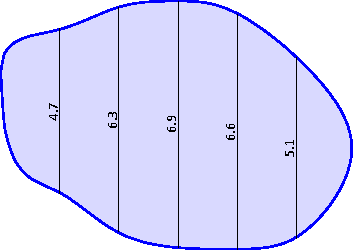
\includegraphics[scale=1]{figures/fig05_05_ex_01}\end{minipage}}

\item {\begin{minipage}{\linewidth}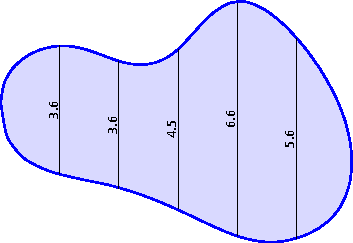
\includegraphics[scale=1]{figures/fig05_05_ex_02}\end{minipage}}

  \item Consider the definite integral $\int_0^1 x \tan(x) \, dx$.
  \ba
  	\item Explain why this integral cannot be evaluated exactly by using either $u$-substitution or by integrating by parts.
	\item Using 4 subintervals, compute $L_4$, $R_4$, $M_4$, $T_4$, and $S_4$.  
	\item Which of the approximations in (b) is an over-estimate to the true value of $\int_0^1 x \tan(x) \, dx$?  Which is an under-estimate?  How do you know?
  \ea
\end{enumerate}

%------------------------------------------
% END OF EXERCISES ON FIRST PAGE
%------------------------------------------
\end{multicols*}
\end{adjustwidth*}

\clearpage

\begin{adjustwidth*}{}{-2.25in}
\setlength{\columnsep}{25pt}
\begin{multicols*}{2}\small

\begin{enumerate}[1),start=27]
  \item For an unknown function $f(x)$, the following information is known.  
  \begin{itemize}
  	\item $f$ is continuous on $[3,6]$;
	\item $f$ is either always increasing or always decreasing on $[3,6]$;
	\item $f$ has the same concavity throughout the interval $[3,6]$;
	\item As approximations to $\int_3^6 f(x) \, dx$, $L_4 = 7.23$, $R_4 = 6.75$, and $M_4 = 7.05$.
  \end{itemize}
  \ba
  	\item Is $f$ increasing or decreasing on $[3,6]$?  What data tells you?
	\item Is $f$ concave up or concave down on $[3,6]$?  Why?
	\item Determine the best possible estimate you can for $\int_3^6 f(x) \, dx$, based on the given information.
  \ea
  
    \item The rate at which water flows through Table Rock Dam on the White River in Branson, MO, is measured in thousands of cubic feet per second (TCFS).  As engineers open the floodgates, flow rates are recorded according to the following chart.
  \begin{center}
\begin{tabular}{|l|c|c|c|c|c|c|c|}
\hline
seconds, $t$ & 0 & 10 & 20 & 30 & 40 & 50 & 60 \\
\hline
flow in TCFS, $r(t)$ & 2000 & 2100 & 2400 & 3000 & 3900 & 5100 & 6500 \\
\hline
\end{tabular}
\end{center}
	\ba
		\item What definite integral measures the total volume of water to flow through the dam in the 60 second time period provided by the table above?
		\item Use the given data to calculate $M_n$ for the largest possible value of $n$ to approximate the integral you stated in (a).  Do you think $M_n$ over- or under-estimates the exact value of the integral?  Why?
		
		\item Approximate the integral stated in (a) by calculating $S_n$ for the largest possible value of $n$, based on the given data.
		
		\item Compute $\frac{1}{60} S_n$ and $\frac{2000+2100+2400+3000+3900+5100+6500}{7}$.  What quantity do both of these values estimate?  Which is a more accurate approximation?
	\ea
\end{enumerate}

%---------------------------------------------
% END OF EXERCISES ON SECOND PAGE
%---------------------------------------------
\end{multicols*}
\end{adjustwidth*}

\afterexercises